\documentclass[authoryear,12pt]{elsarticle}
\makeatletter
\def\ps@pprintTitle{%
 \let\@oddhead\@empty
 \let\@evenhead\@empty
 \def\@oddfoot{\centerline{\thepage}}%
 \let\@evenfoot\@oddfoot}
\makeatother

\makeatletter
\let\@afterindenttrue\@afterindentfalse
\makeatother

\usepackage{listings}
\usepackage{graphicx}
\usepackage{subcaption}
\usepackage{mathtools}
\usepackage{amsthm}
\usepackage{geometry}
\usepackage[authoryear]{natbib}
\usepackage{cleveref}
\bibliographystyle{elsarticle-harv}
\setcitestyle{square}
\geometry{
 left=20mm,
 right=20mm,
 top=20mm,
 bottom=20mm,
 }

\begin{document}
	\begin{frontmatter}
		\title{Solving a singular integral equation using Chebyshev Polynomial Approximation}
		\begin{abstract}
			Broberg \citep{Broberg199999}  derived an equation for the variation of elastostatic crack aperture with the prescribed stress on the crack faces. In this report, we attempt to solve that equation to obtain the relation between crack aperture \(v(x)\) and distance \(x\).
		\end{abstract}
		
		\author{Harshit Garg - 2013A4PS332G}
		
	\end{frontmatter}
	\section{Introduction}
	
		The equation which we attempt to solve is 
		
		\begin{equation*}
			\frac{\partial v(x)}{\partial x} = \frac{-1}{2(1-k^2)G\sqrt{(x-b)(c-x)}}\left\{ \frac{1}{\pi}\int\limits_{b}^c \frac{\sigma_y^0(\xi)\sqrt{(\xi-b)(c-\xi)}}{\xi-x}\,d\xi \,\,+\,\, \sigma^{\infty}_{yy}[x-\frac{b+c}{2}]\right\}
		\end{equation*}
		Here, \(v(x)\) is opening of the crack.
		
	\section{Numerical Solution using Chebyshev Approximation}
	
		\begin{equation}\label{2}
			\frac{\partial v(x)}{\partial x} = \frac{-1}{2(1-k^2)G\sqrt{(x-b)(c-x)}}\left\{ \frac{1}{\pi}\int\limits_{b}^c \frac{\sigma_y^0(\xi)\sqrt{(\xi-b)(c-\xi)}}{\xi-x}\,d\xi \,\,+\,\, \sigma^{\infty}_{yy}[x-\frac{b+c}{2}]\right\}
		\end{equation}
		\\
		as crack extends from \(-a\) to \(a\), replacing \(b\,=\,-a\) \& \(c\, =\,a \) in \cref{2} and integrating from \( -a\,\, to\,\, x \). The singular integral equation which we will get is,
		
		\begin{equation*}
			v(x) = \frac{-1}{2(1-k^2)G}\left \{\frac{1}{\pi}\,\int\limits_{-a}^x \frac{1}{\sqrt{a^2\,-\,x^2}}\left[\int\limits_{-a}^a \frac{\sigma_y^0(\xi)\sqrt{a^2\,-\,\xi^2}}{\xi-x}d\xi\right]dx \,\,+\,\, \int\limits_{-a}^x \frac{\sigma^{\infty}_{yy}\,x}{\sqrt{a^2-x^2}}\,dx\right\}
		\end{equation*}
		\\
		Taking linear relation between stress and crack aperture, i.e. \(\sigma_y^0(\xi)\,=\,2\alpha v(\xi)\), we get,
		\begin{equation}\label{3}
			v(x) = \frac{-1}{2(1-k^2)G}\left \{\frac{2\alpha}{\pi}\,\int\limits_{-a}^x \frac{1}{\sqrt{a^2\,-\,x^2}}\left[\int\limits_{-a}^a \frac{v(\xi)\sqrt{a^2\,-\,\xi^2}}{\xi-x}d\xi\right]dx \,\,+\,\, \int\limits_{-a}^x \frac{\sigma^{\infty}_{yy}\,x}{\sqrt{a^2-x^2}}\,dx\right\}
		\end{equation}\\
		\\
		\\
		There is a Cauchy singularity in the first term of RHS of \cref{3} which have to be removed,
		\begin{equation}\label{4}
			\int\limits_{-a}^a \frac{v(\xi)\sqrt{a^2 - \xi ^2}}{\xi - x}\,d\xi
		\end{equation}
		\\
		To remove this singularity we will use analytical relations defined for Chebyshev Polynomials. For that we will use Chebyshev Approximation. \\ We will approximate \(v(x)\) as linear combination of \(N\) Chebyshev Polynomials with degrees \(0\) to \( N \),
		\begin{equation}\label{5}
			v(x)\,\approx\,\sum\limits_{n=0}^{N} b_n U_n(x)
		\end{equation}
		\\
		where \(U_k(x)\) is Chebyshev Polynomial of second kind of degree k. And \(b_k\)'s will be in \([-1,1]\).
		\\
		Substituting \cref{5} in \cref{3}, we will get,
		\begin{equation*}
			\sum_{n=0}^{N} b_n U_n(x)\,\approx\,\frac{-1}{2(1-k^2)G}\left\{\frac{2\alpha}{\pi}\int\limits_{-a}^x\frac{1}{\sqrt{a^2 - x^2}}\,\left[\int\limits_{-a}^a\frac{\sum\limits_{n=0}^{N} b_n U_n(\xi)\sqrt{a^2-\xi^2}}{\xi-x}\,d\xi \right]\,dx\,+\,\int_{-a}^x \frac{\sigma^{\infty}_{yy}x}{\sqrt{a^2-x^2}}\,dx\right\}
		\end{equation*}
		\\
		Re-arranging,
		\begin{equation}\label{6}
			\sum_{n=0}^{N} b_n U_n(\xi)\,\approx\,\frac{-1}{2(1-k^2)G}\left\{\frac{2\alpha}{\pi}\,\sum_{n=0}^{N}\,\int\limits_{-a}^x\frac{b_n}{\sqrt{a^2 - x^2}}\left[\,\int\limits_{-a}^a \frac{U_n(\xi)\,\sqrt{a^2 - \xi ^2}}{\xi-x}\,d\xi\right] dx\,+\,\sigma^{\infty}_{yy}\int_{-a}^x \frac{x}{\sqrt{a^2-x^2}}\,dx\right\}
		\end{equation}
		\\
		Using Relation between Chebyshev Polynomials \(T_{n}(\xi)\) and \(U_{n}(\xi)\) \citep{cheby},
		\begin{equation*}
			\int_{-1}^1\,\frac{U_n(\xi) \sqrt{1-\xi^2}}{\xi-x}\,d\xi\,=\,-\pi T_{n+1}(x)
		\end{equation*}
		\\
		where \(T_{k}(x)\) is Chebyshev Polynomial of first kind of degree \(k\).
		\\
		\\
		Here we have, 
		\begin{equation}\label{7}
			\int\limits_{-a}^a \frac{U_n(\xi)\,\sqrt{a^2 - \xi^2}}{\xi-x}\,d\xi
		\end{equation}
		\\
		Substituting \(\xi\) to \(a\xi\) in \cref{7} we get,
		\begin{equation}\label{8}
			\int\limits_{-1}^1 \frac{U_n(a\xi)\,\sqrt{a^2 - a^2 \xi ^2}}{a \xi-x}\,a d\xi \,=\, a \int\limits_{-1}^1 \frac{U_n(a\xi)\,\sqrt{1 - \xi^2}}{\xi-\frac{x}{a}}\, d\xi \,=\,-a\pi T_{n+1}(x)
		\end{equation}
		\\
		Substituting \eqref{8} in \eqref{6},
		\begin{equation*}
			\sum_{n=0}^{N} b_n U_n(x)\,\approx\,\frac{-1}{2(1-k^2)G}\left\{\frac{2\alpha}{\pi}\,\sum\limits_{n=0}^{N}\,\int\limits_{-a}^x\frac{b_n}{\sqrt{a^2 - x^2}}\,\left[-a \pi T_{n+1}(x) \right]\,dx\,\,+\,\sigma^{\infty}_{yy}\int_{-a}^x \frac{x}{\sqrt{a^2-x^2}}\,dx\right\}
		\end{equation*}
		\\
		Re-arranging,
		\begin{equation}\label{9}
			\sum_{n=0}^{N} b_n U_n(x)\,=\,\,\frac{a \alpha}{(1-k^2)G}\,\sum_{n=0}^{N}\,\int\limits_{-a}^x\frac{b_n\, T_{n+1}(x)}{\sqrt{a^2 - x^2}}\,dx\,-\,\frac{\sigma^{\infty}_{yy}}{2(1-k^2)G}\int\limits_{-a}^x \frac{x}{\sqrt{a^2-x^2}}\,dx
		\end{equation}
		\\
		we can evaluate the second integral of \cref{9} directly,
		\begin{equation}\label{10}
			\int_{-a}^x \frac{x}{\sqrt{a^2-x^2}}\,dx\,=-\,\sqrt{a^2-x^2}
		\end{equation}
		\\
		Substituting \cref{10} in \cref{9} and also \(\frac{a\alpha}{G} = \alpha^*\),
		\begin{equation*}
			\sum_{n=0}^{N} b_n U_n(x)\,=\,\frac{\alpha^*}{(1-k^2)}\,\sum_{n=0}^{N}\,b_n\,\int\limits_{-a}^x\frac{\, T_{n+1}(x)}{\sqrt{a^2 - x^2}}\,dx \,+\,\frac{\sigma^{\infty}_{yy}\,\sqrt{a^2-x^2}}{2(1-k^2)G}
		\end{equation*}
		\\
		Re-arranging
		\begin{equation}\label{11}
			\boxed{\sum_{n=0}^{N} b_n \bigg(U_n(x)\,-\,\frac{\alpha^*}{(1-k^2)}\,\int\limits_{-a}^x\frac{\, T_{n+1}(x)}{\sqrt{a^2 - x^2}}\,dx\bigg)\,=\,\frac{\sigma^{\infty}_{yy}}{2(1-k^2)G}\,\sqrt{a^2-x^2}}
		\end{equation}
		\\
		Code for solving this equation numerically is given in Appendix- A which take crack-half length\(\,=\,a\, , \,\alpha^*\, , \,G\, , \,k\, , \,\sigma^{\infty}_{yy}\) as input.
	\\
	\\
	\section{Comparision with Perturbation Solution}
	An exact formulation is known for the crack aperture in the presence of a known spatially-variable normal hydrostatic pressure acting along the crack faces \citep{sneddon1969crack}. The present problem is different, in the sense that the cohesive stress is not known. A regular perturbation technique \citep{hinch1991perturbation} will be utilised to address the problem. The classical solution for the case of no cohesive force will be taken as the zeroth-order solution. The aperture that is obtained in the zeroth-order solution is then used to calculate the cohesive force, according to the law \(\sigma_y^0(\xi)\,=\,2\alpha v(\xi)\). This force is then applied to the surfaces of the crack, and Sneddon's formulation is used to calculate the additional crack aperture and stress field due to this surface force. This new incremental aperture will give rise to an additional cohesive force and so this process would need to be iterated until convergence is obtained. Convergence of this perturbation process could be defined. for example, as the stage at which the incremental aperture compute at step N is less than some prescribed fraction of the zeroth-order aperture. For simplicity, only one step of this iterative process will be considered, which is expected to be sufficient for validating the accuracy of the numerical solution procedure.
	
	
	For the case of a spatially variable pressure acting on the crack face, the aperture variable for the zeroth-order solution plus the first-order perturbation correction can be written as \citep{sneddon1969crack}
	
	\begin{equation}\label{12}
		v_{sn}(x)\,=\,\frac{2p_0(1-\nu^2)a}{E}\left[\sqrt{1-\left(x^2/a^2\right)}-\frac{2(1-\nu^2)a}{E}\,\int\limits_{x/a}^1 \frac{tq(t)}{\sqrt{t^2-(x/a)^2}}\,dt\right]
	\end{equation}
	where,
	
	\begin{equation} \label{13}
		q(t) = \frac{2}{\pi}\int\limits_{0}^t \frac{p(u)/p_{0}}{\sqrt{t^2-u^2}}\,du
	\end{equation}
	
	with,
	\begin{equation} \label{14}
		p(u) = 2\alpha p_{0}\sqrt{1-\left(u^2/a^2\right)}	
	\end{equation}\\
	Here,crack-half length is \(a\), Young's Modulus \(E\), and Poisson's Ration \(\nu\).
	\\
	\\
	for chebyshev approximation solution we use condition \(\sigma^{\infty}_{yy} \,=\, 1  \) and\\
	for perturbation solution we use condition \(p_0 = 1\).\\
	These both condtions are same as [Reason i don't know]
	
	\newpage
	\section{Results}
		\subsection{Crack Aperture}
			A line crack that extends from \(b = -a\) to \(c = a\) with \(a = 1\) (for concrete numerical purposes). is considered. Validation of the numerical results can be done by comparision with the first order perturbation solution. The two approaches should closely agree for small values of \(\alpha\), which can be expressed in dimensionless form as \(\alpha ^{*}\,=\,\alpha a /G \) \\
		\begin{figure}[h!]
            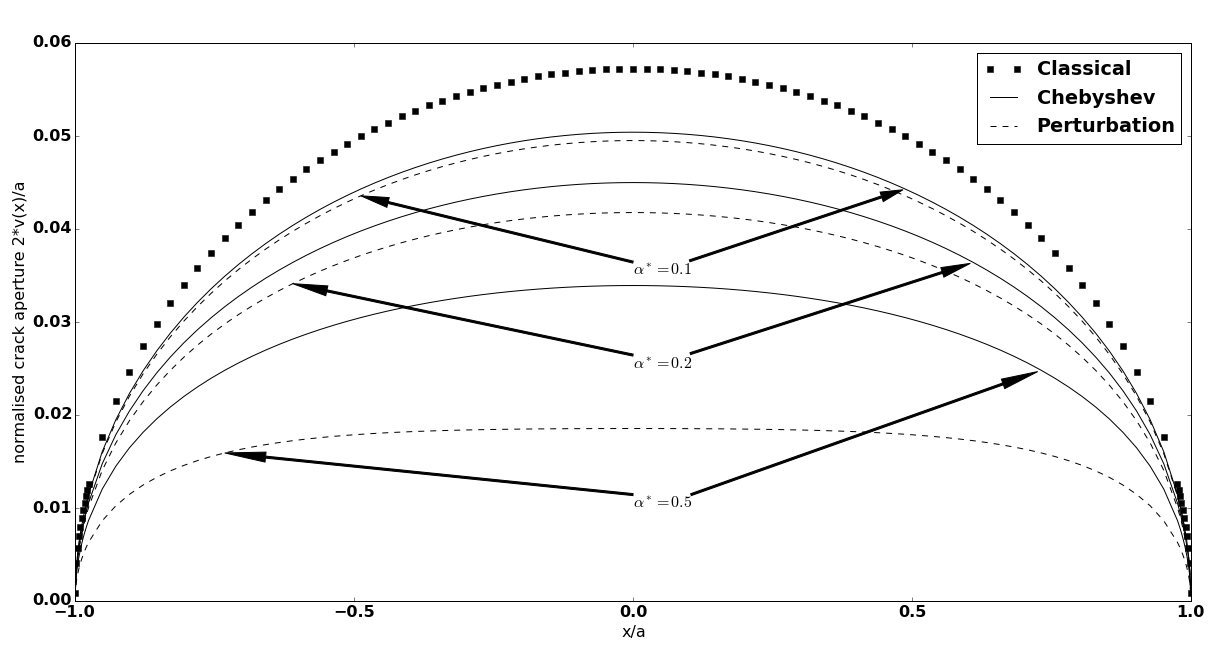
\includegraphics[width=1\linewidth]{Result.png}
            \caption{Crack face separation in presence of cohesive stress with parameter \(\alpha^*\) when applied load is \(\sigma_{yy}^{\infty}\)}
			\label{Result}
        \end{figure}
		\\
    As can be observed in \cref{Result}, for small values of \(\alpha^*\), the perturbation solution agrees closely with the full cohesive stress solution. As \(\alpha^*\) is increased, the perturbation solution becomes less accurate, so that for \(\alpha^*\) = 0.5 and beyond, the comparision are no longer meaningful.
	\newpage
	\subsection{Error}
		A further test to validate the results is to track the error in the calculation of correction aperture in the cohesive solution at the mid point of crack i.e \(x-0\).
		\begin{equation*}
			Error_{x=0} = \frac{(Aperture_{Cohesive}\,-\,Aperture_{Perturbation})_{x=0}}{(Aperture_{Classical}\,-\,Aperture_{Perturbation})_{x=0}}
		\end{equation*}
		\\
		\begin{figure}[h!]
            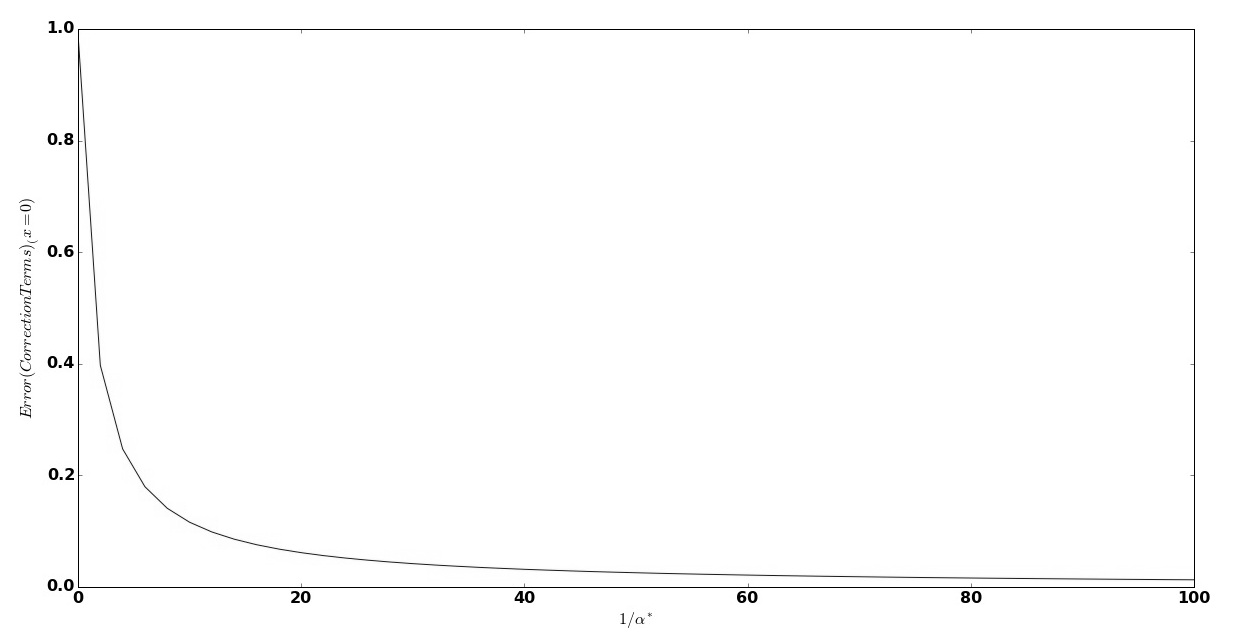
\includegraphics[width=1\linewidth]{Error.jpg}
            \caption{Variation of Error at \(x \,=\, 0\) between the Chebyshev cohesive solution and the first order perturbation solution as a function of \(\alpha^*\)}
			\label{Error}
		\end{figure}
		\\
		As can be observed from \cref{Error}, the error reduces as \(\alpha^*\) decreases which implies that as \(\alpha^*\) decreases perturbation solution comes closer to cohesive solution.
	\newpage
	\subsection{Stress Along the Crack Line}
		After the aperture \((2v_{+})\) and cohesive stress \(\sigma^{0}_{y}(\xi)\,=\,2\alpha v_{+}(\xi)\) have been calculated.
		\begin{equation}\label{15}
			\sigma_y = 2\Re p'(x) = \pm \frac{1}{\sqrt{(x-b)(x-c)}}\left\{ \frac{1}{\pi}\int\limits_{b}^c \frac{\sigma_y^0(\xi)\sqrt{(\xi-b)(c-\xi)}}{\xi-x}\,d\xi \,\,+\,\, \sigma^{\infty}_{yy}[x-\frac{b+c}{2}]\right\}
		\end{equation}
		\\
		\cref{15} can be solved for the stress \(\sigma_{yy}\) along the crack line.\\

		\begin{figure}[!]
			\begin{subfigure}{1\textwidth}
				\begin{center}
					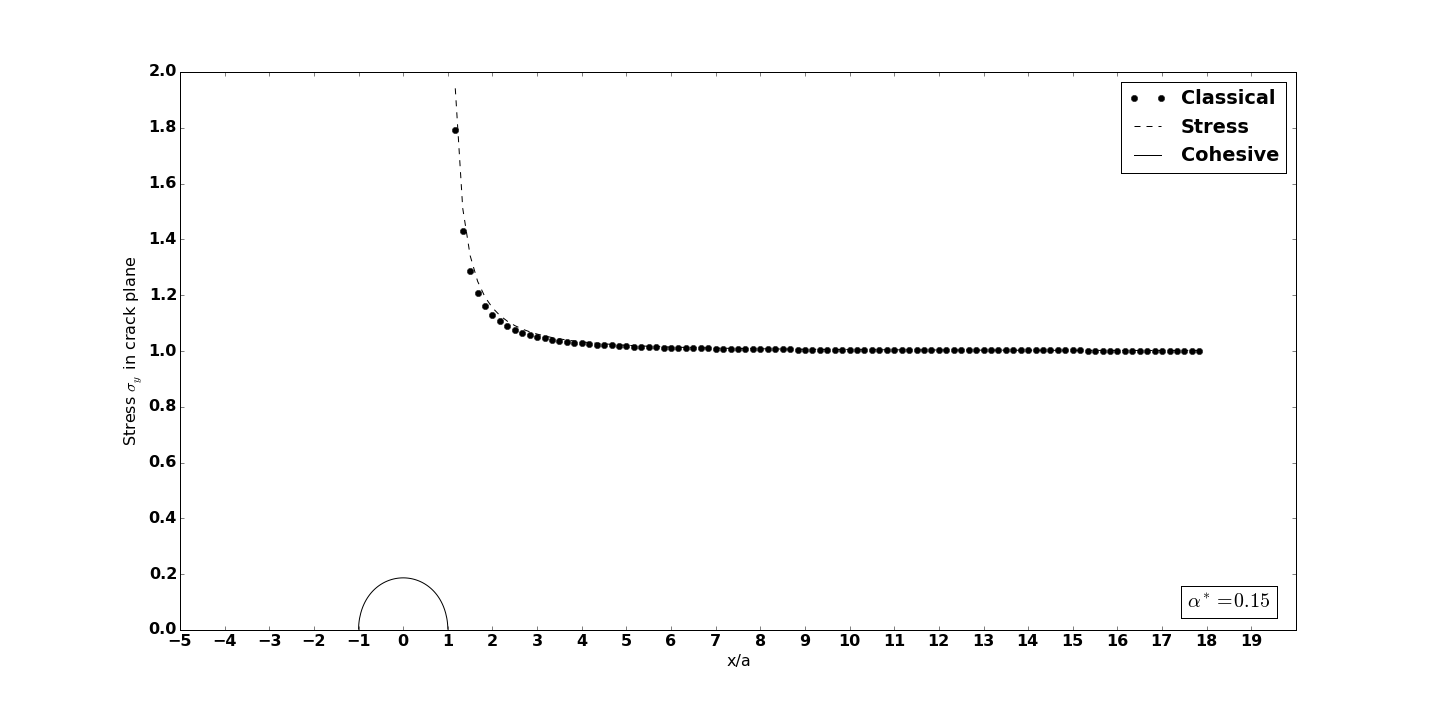
\includegraphics[width=1.15\linewidth]{Stress_1.png}
				\end{center}
				\caption{}
			\end{subfigure}
			\begin{subfigure}{1\textwidth}
				\begin{center}
					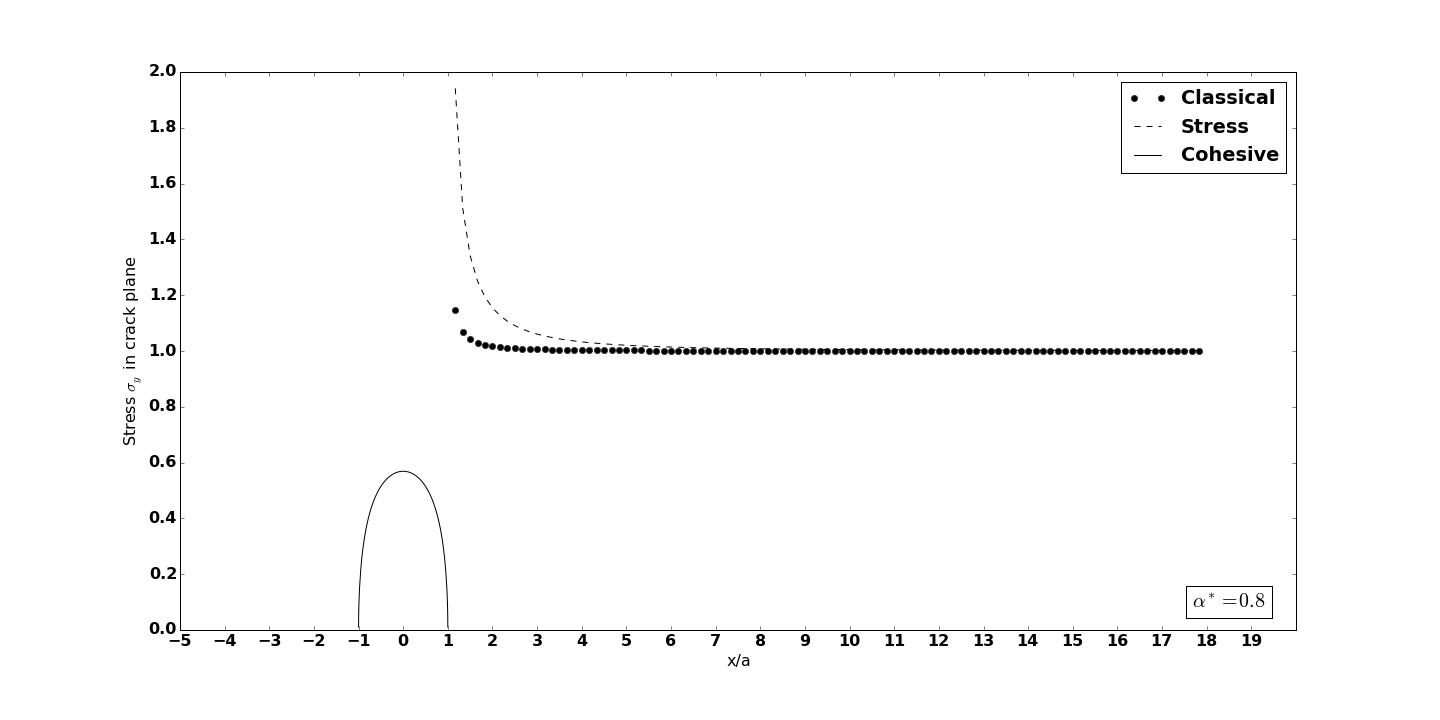
\includegraphics[width=1.15\linewidth]{Stress_2.png}
				\end{center}
				\caption{}
			\end{subfigure}
			\caption{Variation of \(\sigma_y\) in \cref{15} across the crack line for different values of cohesive stress}
		\end{figure}	
		\newpage
		\section{Appendix}
		\lstinputlisting[language=Python]{SOP_Linear.py}
		\newpage
\bibliography{Bibliography}
\end{document}